\chapter{提案手法の実装とシミュレーションの環境}
\label{chap:implementation_and_experimentation}

\section{Omnet++とDTNsimを用いた評価環境}
Omnet++はネットワークシミュレータの構築を目的としたオープンソースのプラットフォームであり、
既存の通信プロトコルや物理層のシミュレーションを実装しているほか、
各ノードにC++でのアプリケーションを実装し拡張することが可能である。
DTNsimはOmnet++のフレームワーク上で動作するDTNのシミュレーターであり、
ION-DTN、HDTNなどの種々のDTN実装が動作するネットワークをシミュレートすることができ、
各種CGRのバリエーションにも対応する。そのため本研究ではこのOmnet++とDTNsimを用いて
宇宙で運用されているDTNをシミュレーションを行う。

\subsection{2040年代のDTNを想定したシナリオとパラメータ}
本実験においては、2040年代の複数の天体間にまたがるDTNを運用していることを想定し、
そのうち任意の2天体間について既存手法と本研究の提案手法の実装とシミュレーションを行い、
本研究の提案の有効性について検証する。そのため任意の2天体間のDTNネットワークとして、
図\ref{fig:experimentation_topology}のようなトポロジーを想定する。
ノード1から3は天体A、ノード4から6はそれぞれ天体Bに属するDTNノードであり、
ノード1と6はそれぞれの地表DTNのノード、ノード2から5はそれぞれの天体の軌道上にある
宇宙のDTNノードである。

\begin{figure}[tbh]
    \centering
    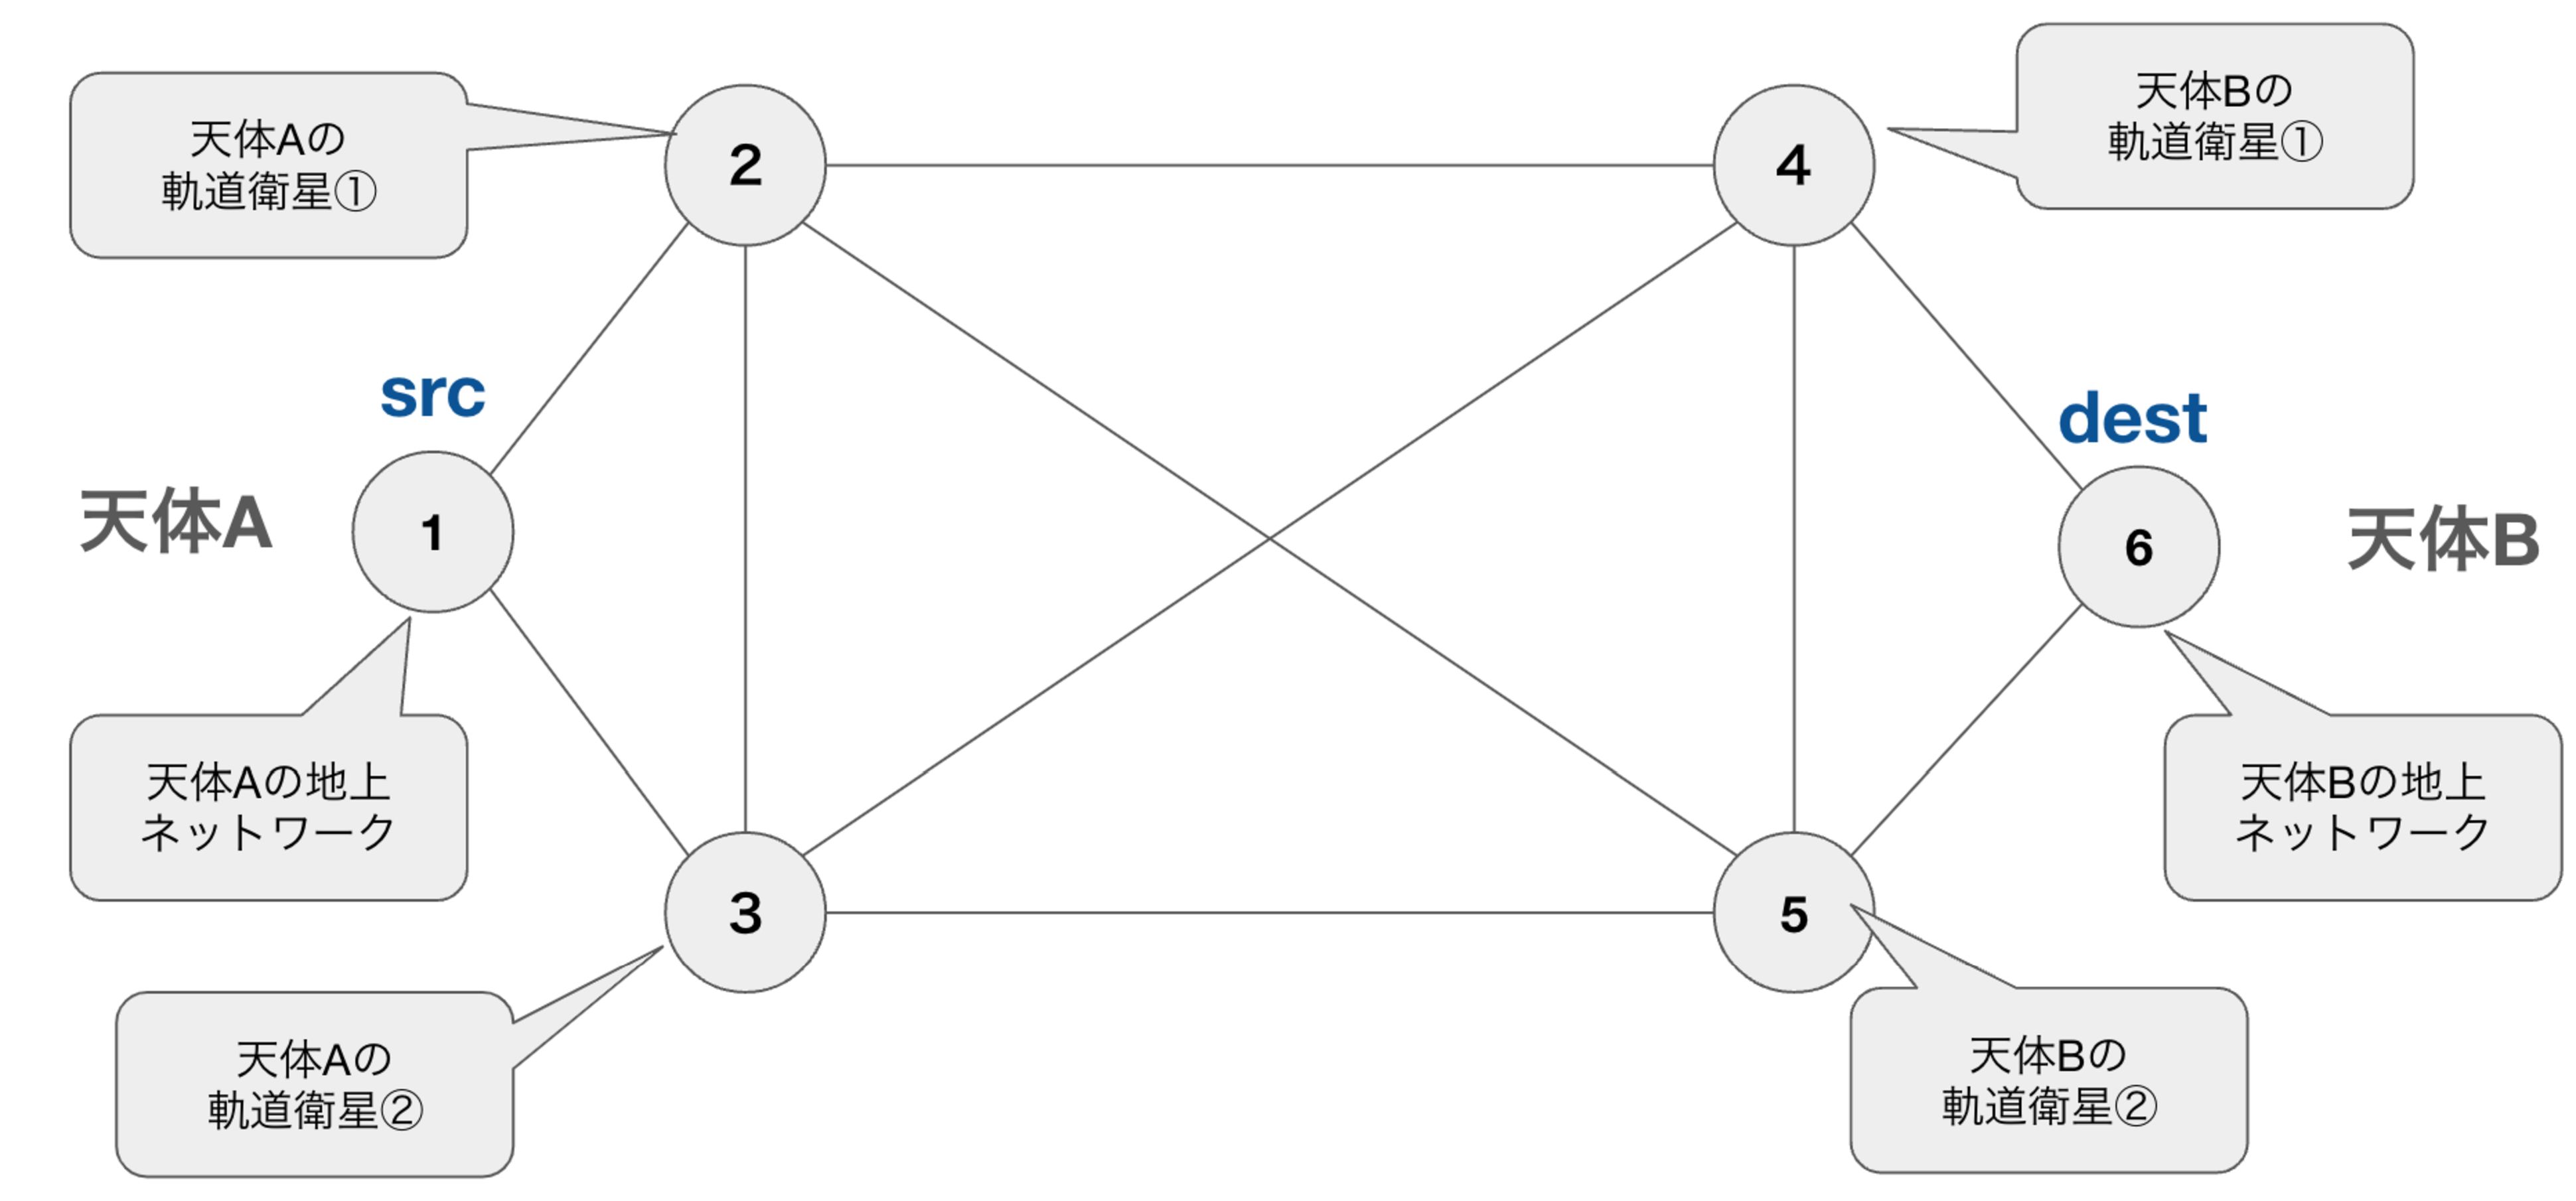
\includegraphics[width=0.7\textheight]{img/thesis_Sample_topology.pdf}
    \caption{本実験で用いるトポロジー}
    \label{fig:experimentation_topology}
    \begin{minipage}{\textwidth}
        \raggedright
        \vspace{3mm}
        ノード1は天体Aの地上DTNネットワークを代表したノード、ノード2とノード3は
        天体Aの軌道上に存在する宇宙のDTNノード、ノード4とノード5は
        天体Bの軌道上に存在する宇宙のDTNノード、
        ノード6は天体Bの地上DTNネットワークを代表したノードを示す。
    \end{minipage}
\end{figure}

\subsection{シミュレーションで用いるバンドルトラフィック}
\label{subsection:シミュレーションで用いるバンドルトラフィック}
本実験では図\ref{fig:experimentation_topology}のトポロジーにおいて、
ノード1からノード6に向かう、すなわち天体Aの地上DTNネットワークから天体Bの地上DTNネットワークに
向けてのトラフィックを想定する。生成するバンドルのトラフィック量は、実験ごとに
ランダムに生成を行っている。ただし生成するバンドルについて、
それぞれ範囲等を絞って生成している。以下にそれぞれを示す。
\begin{itemize}
    \item バンドル生成イベントごとのバンドルの生成数(bundlesNumber)
    \item バンドル生成イベントの開始タイミング(start)
    \item 生成したバンドルの目標ノードのendpoint ID(destinationEid)
    \item バンドル生成イベントごとのバンドルのサイズ(size)
\end{itemize}
\subsection{リンク障害のシナリオ生成}
リンク障害のシナリオ作成には、omnetppで実装されているFaultサブモジュールを用いる。
\section{Contact Planの臨時更新の実装}
Contact Planからのリンクの削除と追加は、omnetppで実装されているCentralサブモジュールを用いる。
